\documentclass[12pt, a4paper, brazil]{abntex2}
\usepackage[utf8]{inputenc}
\usepackage[T1]{fontenc}
\usepackage[left=2cm, top=3cm, right=2cm, bottom=2cm]{geometry}
\usepackage[normalem]{ulem}
\usepackage[dvipsnames]{xcolor}
\usepackage{graphicx}
\graphicspath{{./src/img/}}
\usepackage{float}

\usepackage[alf]{abntex2cite}

\usepackage{hyperref}
\hypersetup{
    colorlinks=true,
  linkcolor=black,
  citecolor=black,
  urlcolor=black
  }

\usepackage[most]{tcolorbox}

\usepackage{indentfirst}
\usepackage{multicol}

\setlength{\columnseprule}{0.5pt}
\setlength{\columnsep}{25pt}

\usepackage{amsmath}
\usepackage{amsthm}
\usepackage{amsfonts}
\usepackage{amssymb}
\usepackage{xfrac}
\usepackage{thmtools}

\usepackage{enumitem}

\DeclareMathOperator{\sen}{sen}
\DeclareMathOperator{\tg}{tg}

\renewenvironment{proof}{\vspace{\onelineskip} \noindent{\bfseries Demonstração:}}{\qed}

\setcounter{tocdepth}{2}

\newcounter{questaovest}

\newcommand{\vest}[1]{\stepcounter{questaovest}\item[\textbf{Questão \arabic{questaovest}}:]}
\setlist[enumerate]{
    align=left,
    leftmargin=*,
    }
    
\setlist[enumerate,2]{
    label=\alph*.,
    font=\bfseries,
    itemsep=0.1pt,
    labelsep=0em,
    parsep=0pt,
    leftmargin=1.2em
    }
    
    
    \renewcommand{\bibsection}{%
  \chapter*[Referências]{Referências} % Na página e no cabeçalho
  \addcontentsline{toc}{chapter}{Referências} % No Sumário
  }

  \chapterstyle{companion}
  \renewcommand{\printchaptertitle}[1]{
  \begin{adjustwidth}{}{0pt}
    \raggedleft\chaptitlefont#1\par\nobreak,
  \end{adjustwidth}
}

%Configuração de Cabeçalho e rodapé
\makepagestyle{myHeader}
\makeoddhead{myHeader}{Pré-Univesitário Social Oficina do Saber / UFF}{}{Matemática: Eduardo}
\makeevenhead{myHeader}{Pré-Univesitário Social Oficina do Saber / UFF}{}{Matemática: Eduardo}
\makeoddfoot{myHeader}{}{-\thepage-}{}
\makeevenfoot{myHeader}{}{-\thepage-}{}
\makeheadrule{myHeader}{\textwidth}{\normalrulethickness}

% --- Customização de Títulos ---
\definecolor{AzulElegante}{RGB}{25, 50, 110}

\renewcommand{\ABNTEXchapterfont}{\rmfamily\bfseries\color{AzulElegante}}
\renewcommand{\ABNTEXsectionfont}{\rmfamily\bfseries\color{AzulElegante}\LARGE\bigskip}
\renewcommand{\ABNTEXsubsectionfont}{\rmfamily\bfseries\color{AzulElegante}}
\renewcommand{\ABNTEXsubsubsectionfont}{\rmfamily\bfseries\color{AzulElegante}}
\renewcommand{\ABNTEXsubsubsubsectionfont}{\rmfamily\bfseries\color{AzulElegante}}
% -------------------------------

\setsecheadstyle{\centering\ABNTEXsectionfont}

%-------- Ambiente de Definição
\newtcolorbox{definicao}[1]{
    colback=gray!25!white,
    colframe=gray!75!black,
    fonttitle=\bfseries,
    title=Definição: #1,
    }
    
    \declaretheoremstyle[
        spaceabove=\topsep,
        spacebelow=\topsep,
        headfont=\bfseries,
        %postheadspace=\newline,
        ]{compactbreak}
    
        \declaretheorem[
            style=compactbreak,
            name=Exemplo
            ]{exemplo}

\begin{document}
  \begin{enumerate}
    \vest{} Converta os ângulos em radianos:
        \begin{enumerate}
            \item 300°
            \item 120°
            \item 135°
        \end{enumerate}
    \vest{} Converta de radianos para ângulos:
        \begin{enumerate}
            \item $\displaystyle\frac{\pi}{12}$ \vspace*{10pt}
            \item $\displaystyle\frac{3\pi}{4}$\vspace*{10pt}
            \item $\displaystyle\frac{7\pi}{4}$\vspace*{10pt}
        \end{enumerate}

    \vest{} Uma praça possui formato circular com 24 metros de diâmetro. Durante o planejamento do evento de inauguração da praça, o prefeito pediu que fosse foi feita uma cerca em todo o comprimento da circunferência, para controlar a entrada dos visitantes desse evento. Qual é o comprimento mínimo de material necessário para cercar toda a praça?
    Considere $\pi = 3$.
    \vspace{4cm}

    \vest{} Kárita decidiu fazer caminhada todos os dias em volta do parque que tem próximo da sua casa. Esse parque conta com um circuito circular, de raio medindo 42 metros. Se, em determinado dia, ela decide andar no mínimo 5 km, o número mínimo de voltas inteiras que ela deve dar em torno desse circuito é igual a: (Considere $\pi=3$)
    \vspace{4cm}
    
    \newpage
    \vest{} As retas t, u e v são paralelas. Determine a medida do segmento x.

        \begin{figure}[H]
            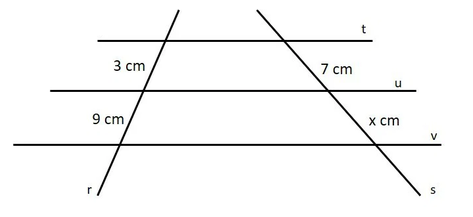
\includegraphics[width=0.4\textwidth]{q05.png}
        \end{figure}
    \vspace*{1cm}

    \vest{}João decidiu dividir um terreno, conforme a imagem abaixo. Determine os valores de a, b e c.
        
        \begin{figure}[H]
            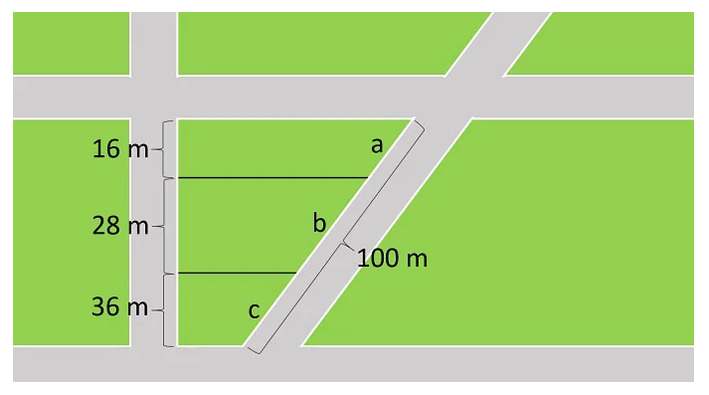
\includegraphics[width=0.4\textwidth]{q06.png}
        \end{figure}
    \vspace*{1cm}

    \vest{} A luz do sol projeta sombras com a mesma angulação em objetos distintos. Podemos utilizar este fato para calcularmos a altura de obtejtos muito altos, somente utilizando a semelhança entre triângulos. Observe a figura a seguir:

        \begin{figure}[H]
            \centering
            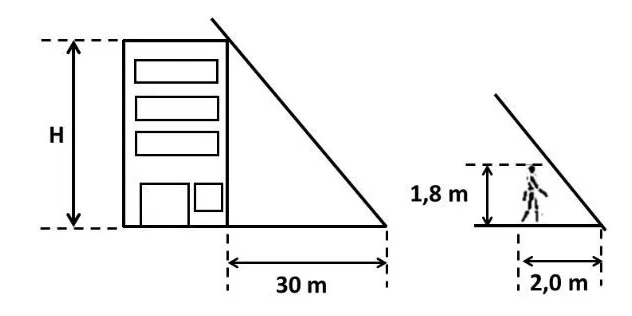
\includegraphics[width=0.4\textwidth]{q07.png}
        \end{figure}

    Se o prédio projeta uma sombra de 30m, no mesmo instante em que um homem de 1,8m projeta uma sombra de 2m, podemos afirmar que a altura deste prédio é:

  \end{enumerate}
\end{document}